\subsection{Logistic regression}
Logistic regression will help us make a 0/1-decision continuous and smooth.

First, we need the \textbf{logisitic function}\sidenote{Logistic function}:
\begin{figure}[H]
  \centering
  \begin{subfigure}{0.3\textwidth}
    \centering
    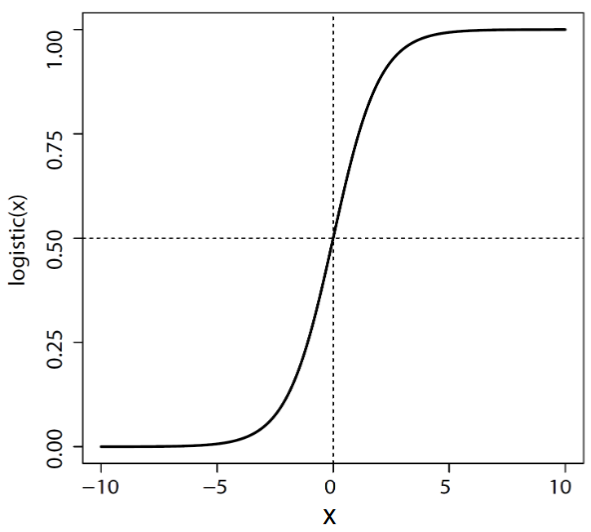
\includegraphics[width=1\textwidth]{assets/regression/lr__log_func.png}
  \end{subfigure}\hspace*{0.05\textwidth}
  \begin{subfigure}{0.6\textwidth}
    \centering
    \begin{align*}\begin{aligned}
      logistic(x) &= \frac{1}{1+e^{-x}}\\
      \frac{d}{dx}logistic(x) &= logistic(x)\cdot\big(1-logistic(x)\big)
    \end{aligned}
    \end{align*}
  \end{subfigure}
  \caption{Logistic function}
  \label{fig:4_logistic_func}
\end{figure}

\begin{itemize}
  \item Here, $e=2.7182818\cdots$ is Eulers number
  \item Any value is mapped on a value between 0 and 1
  \begin{note}\begin{itemize}
    \item $logistic(0)=0.5$, $logistic(-\infty)=0$, $logistic(+\infty)=1$
  \end{itemize}\end{note}
  \item 0 and 1 are quickly approached, therefore we can use it as a "smooth binary value"
\end{itemize}

So now, we can use \textbf{logistic regression}\sidenote{Logistic regression} instead of a hard 0/1-decision.
\begin{figure}[H]
  \centering
  \begin{subfigure}{0.4\textwidth}
    \centering
    \vspace*{0.5cm}

    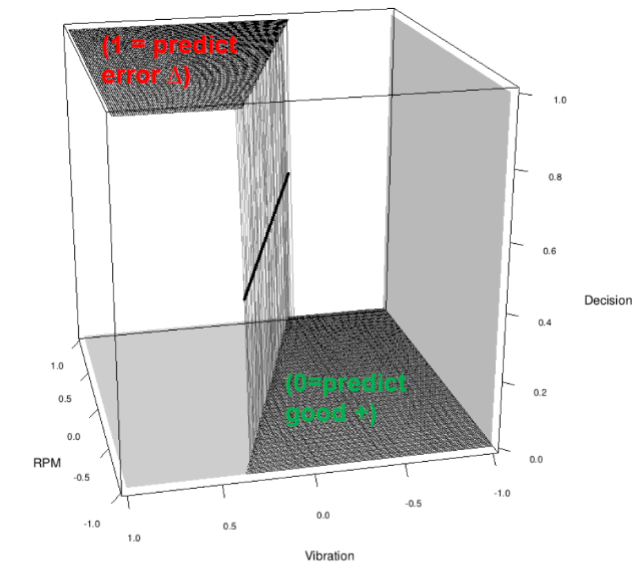
\includegraphics[width=1\textwidth]{assets/regression/lr__01.png}
    \begin{align*}
      \mathbb{M}_\mathbf{w}(\mathbf{d}) = 
        \left\{\begin{array}{ll} 
          1& \text{if }\mathbf{w}\cdot\mathbf{d}\geq0\\
          0& \text{otherwise}
        \end{array}\right.
    \end{align*}
  \end{subfigure}\hspace*{0.05\textwidth}$\rightarrow$\hspace*{0.05\textwidth}
  \begin{subfigure}{0.4\textwidth}
    \centering
    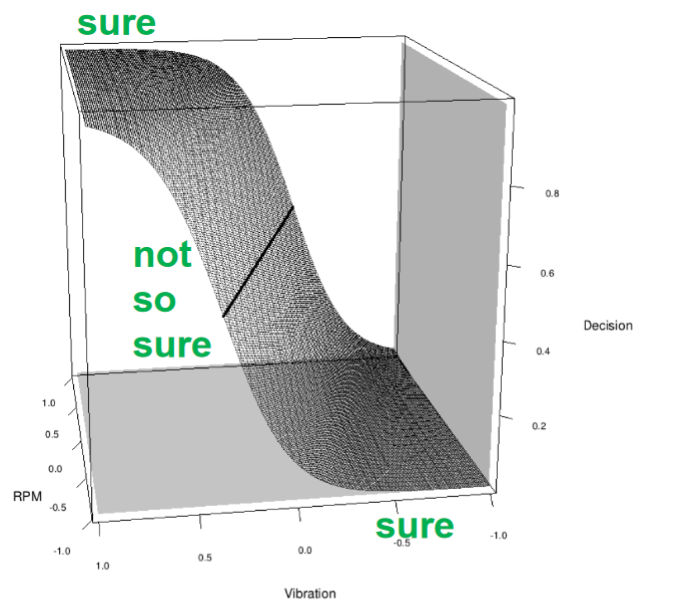
\includegraphics[width=1\textwidth]{assets/regression/lr__logistic.png}
    \begin{align*}
      \mathbb{M}_\mathbf{w}(\mathbf{d}) = logistic(\mathbf{w}\cdot\mathbf{d})
    \end{align*}
  \end{subfigure}
  \caption{Difference 0/1 and logistic}
  \label{fig:4_difference_01_logistic}
\end{figure}

The probabilistic interpretation looks as follows:
\begin{itemize}
  \item $P[t='\text{faulty}' \mid \mathbf{d}] = \mathbb{M}_\mathbf{w}(\mathbf{d})$
  \item $P[t='\text{good}' \mid \mathbf{d}] = 1 - \mathbb{M}_\mathbf{w}(\mathbf{d})$
  \item And the system is more sure about the decision, the further it is away from the separating line.
\end{itemize}
